\documentclass{article}

% Conditional compilation.
% NOTE: If you set fullversionfalse, just compile ONCE so that TOC stays unchanged.
\newif\iffullversion
\fullversiontrue
%\fullversionfalse


%%%%%%%%%%%%%%%%%%%%%%%%%%%%%%%%%%%%%%%%%%%%%%%%%%%%%%%%%%%%%%%%%%%%%%%%%
\pagestyle{plain}                                                      %%
%%%%%%%%%% EXACT 1in MARGINS %%%%%%%                                   %%
\setlength{\textwidth}{6.5in}     %%                                   %%
\setlength{\oddsidemargin}{0in}   %% (It is recommended that you       %%
\setlength{\evensidemargin}{0in}  %%  not change these parameters,     %%
\setlength{\textheight}{8.5in}    %%  at the risk of having your       %%
\setlength{\topmargin}{0in}       %%  proposal dismissed on the basis  %%
\setlength{\headheight}{0in}      %%  of incorrect formatting!!!)      %%
\setlength{\headsep}{0in}         %%                                   %%
\setlength{\footskip}{.5in}       %%                                   %%
%%%%%%%%%%%%%%%%%%%%%%%%%%%%%%%%%%%%                                   %%
\newcommand{\required}[1]{\section*{\hfil #1\hfil}}                    %%
\renewcommand{\refname}{\hfil References Cited\hfil}                   %%
\bibliographystyle{plain}                                              %%
%%%%%%%%%%%%%%%%%%%%%%%%%%%%%%%%%%%%%%%%%%%%%%%%%%%%%%%%%%%%%%%%%%%%%%%%%

\usepackage{graphicx}
\usepackage{color}

\pagestyle{empty}


\usepackage{fancyvrb}

\newenvironment{bluecode}{\VerbatimEnvironment \color{blue} \begin{Verbatim}}
{\end{Verbatim}}


\begin{document}

\large

\vbox{}
\begin{figure}[!ht]
%\hspace{-4mm}

\includegraphics[width=8cm]{img/logo.png}
\vspace{18mm}
\end{figure}

\begin{figure}[!ht]
\begin{center}
%\hspace{-4mm}
%\hspace{-20mm}
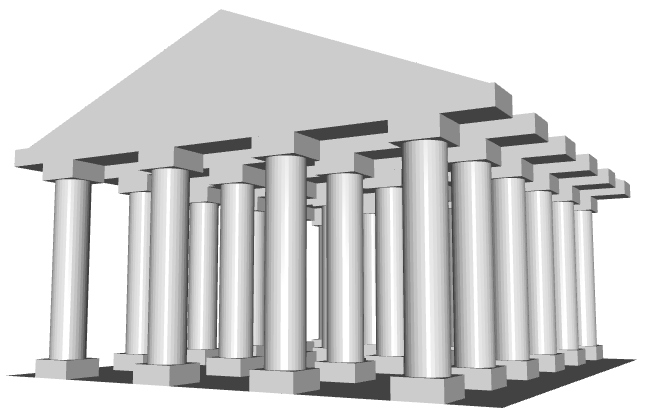
\includegraphics[width=8cm]{img/plasm-temple.png}\hspace{1cm}
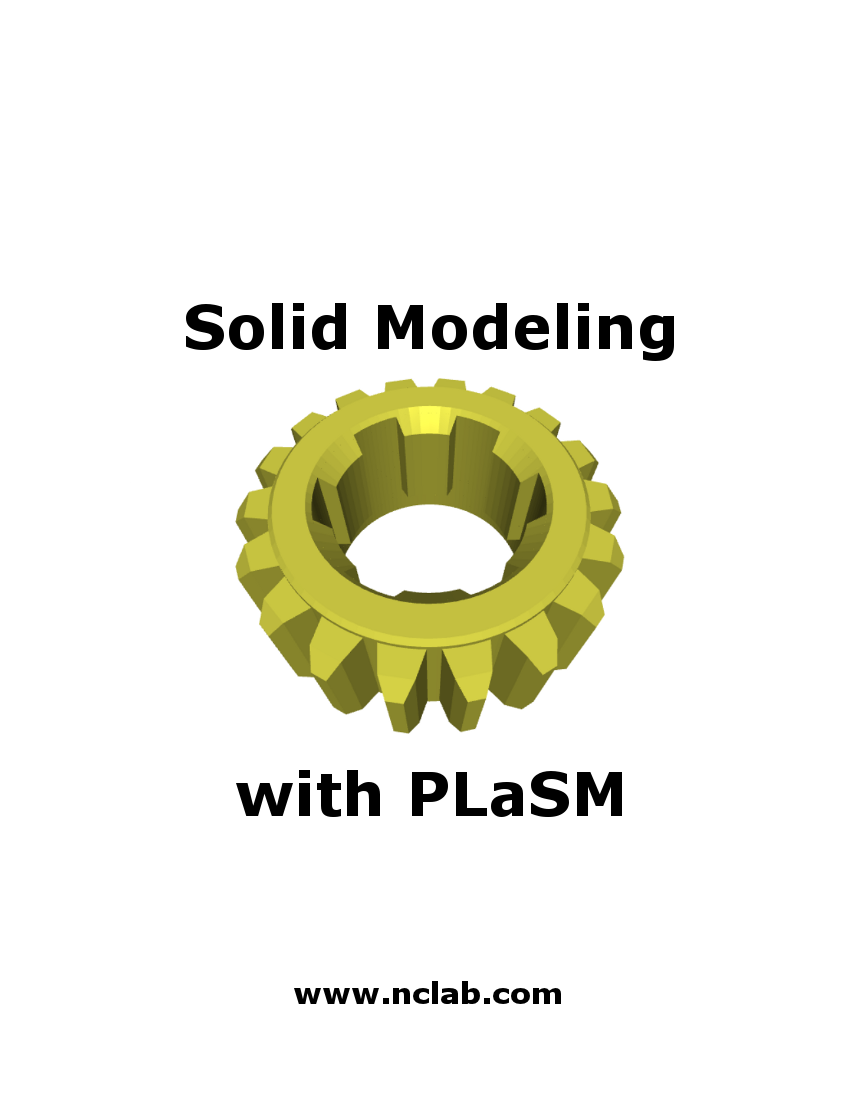
\includegraphics[width=5.5cm]{img/plasm-frontpage.png}
\vspace{15mm}
\end{center}
\end{figure}

\begin{center}
{\Huge \bf Exercises}\\
\vbox{}
\vspace{1.4cm}
\iffullversion
\else
\centerline{\huge \color{red}{PREVIEW}}
\fi
\vfill
{\large
{\bf Pavel Solin \& Alberto Paoluzzi}
}
\end{center}
\vfill
\vfill
\begin{center}
Copyright 2012 FEMhub Inc. All rights reserved.
\end{center}
\newpage
\hbox{}
%%%%%%%%%%%%%%%%%%%%%%%%%%%%%%%%%%%%%%%%%%%%%%%%%%%%%%%%%%%%%%%%%%%%%%%%%


\newpage
%{\ }
\setcounter{tocdepth}{2}
\tableofcontents
%\pagestyle{plain}


%%%%%%%%%%%%%%%%%%%%%%%%%%%%%%%%%%%%%%%%%%%%%%%%%%%%%%%%%%%%%%%%%%%%%%%%%
\newpage

\pagestyle{plain}
\setcounter{page}{1}

\section{Getting Started}

\subsection{Exercises}

\begin{enumerate}
\item Write a script to render a unit cube in darkest pure red color.
\item Write a script to render a unit cube in lightest pure red color.
\item Write a script to render a cube of edge length 2 in darkest pure green color.
\item Write a script to render a cube of edge length 2 in lightest pure green color.
\item Write a script to render a cube of edge length 3 in darkest pure blue color.
\item Write a script to render a cube of edge length 3 in lightest pure blue color.
\end{enumerate}

\section{Creating Simple Objects}

\subsection{Exercises}

\begin{enumerate}
\item
Create a $3 \times 4 \times 5$ brick in a light
blue color, as shown in Fig. \ref{fig:a1}.

\newpage

\begin{figure}[!ht]
\begin{center}
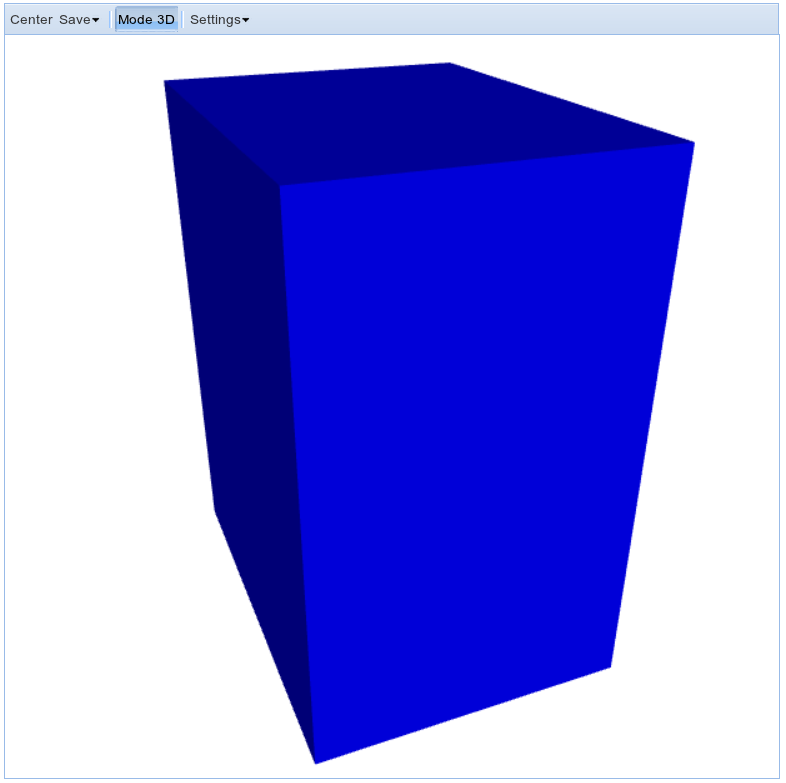
\includegraphics[width=0.5\textwidth]{img/a1-blue-brick.png}
\end{center}
\vspace{-2mm}
\caption{Illustration for Exercise 1.}
\label{fig:a1}
%\vspace{-1cm}
\end{figure}

\item Create a $3 \times 1$ rectangle in a light
red color, as shown in Fig. \ref{fig:a2}.

\begin{figure}[!ht]
\begin{center}
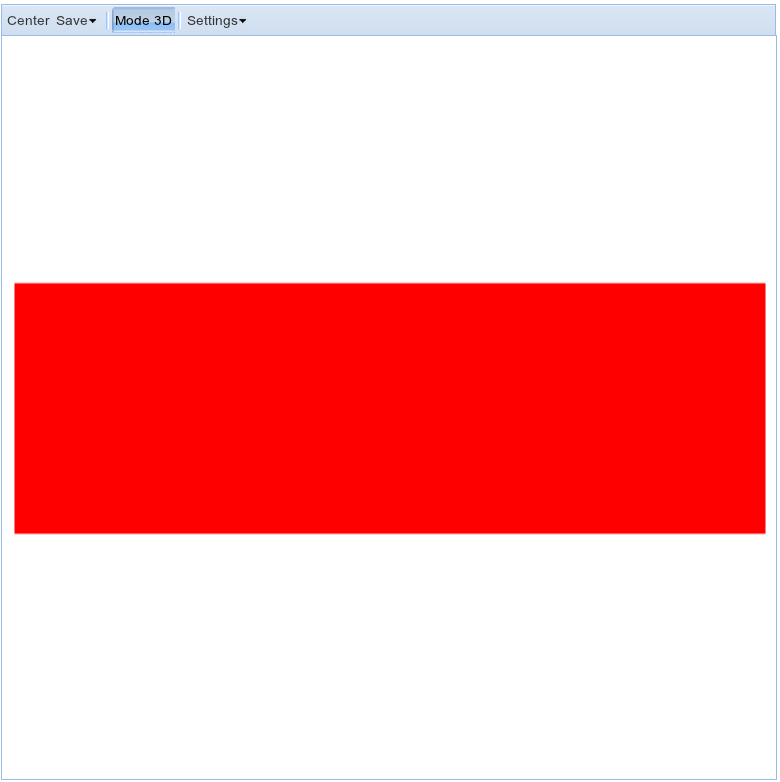
\includegraphics[width=0.5\textwidth]{img/a2-red-rectangle.png}
\end{center}
\vspace{-2mm}
\caption{Illustration for Exercise 2.}
\label{fig:a2}
\vspace{-0cm}
\end{figure}

\item Create an orange octahedron with vertices 
(0, -1, 1), (0, 1, 1), (0, -1, -1), (0, 1, -1), (2, 0, 0), and (-2, 0, 0), 
as shown in Fig. \ref{fig:a3}.

\begin{figure}[!ht]
\begin{center}
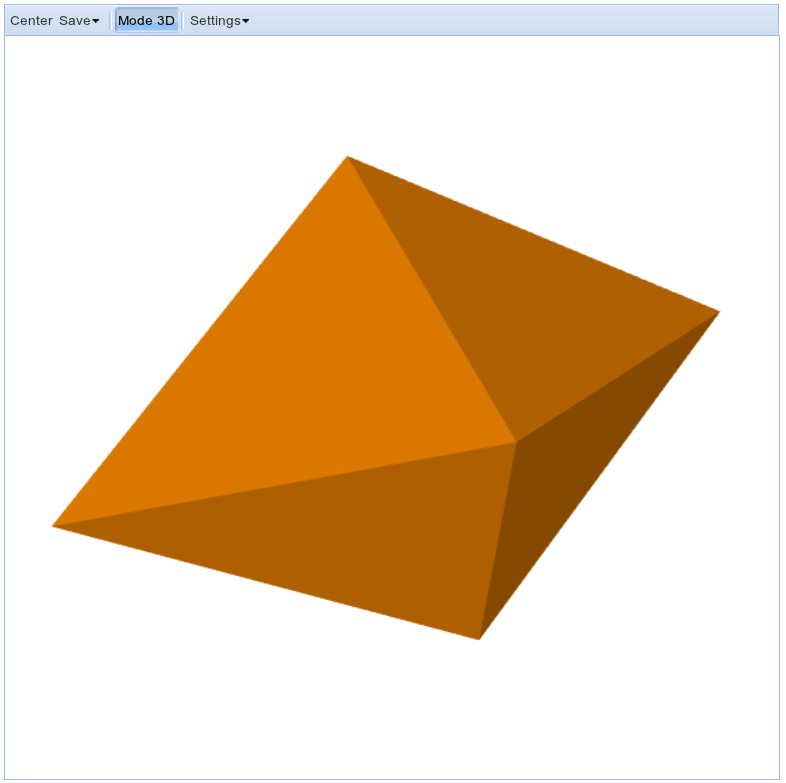
\includegraphics[width=0.5\textwidth]{img/a3-orange-octahedron.png}
\end{center}
\vspace{-2mm}
\caption{Illustration for Exercise 3.}
\label{fig:a3}
%\vspace{-1cm}
\end{figure}

\item Create a pink pentagon with equally-long edges that is inscribed 
in a circle with diameter $R$, as shown in Fig. \ref{fig:a4}.

\begin{figure}[!ht]
\begin{center}
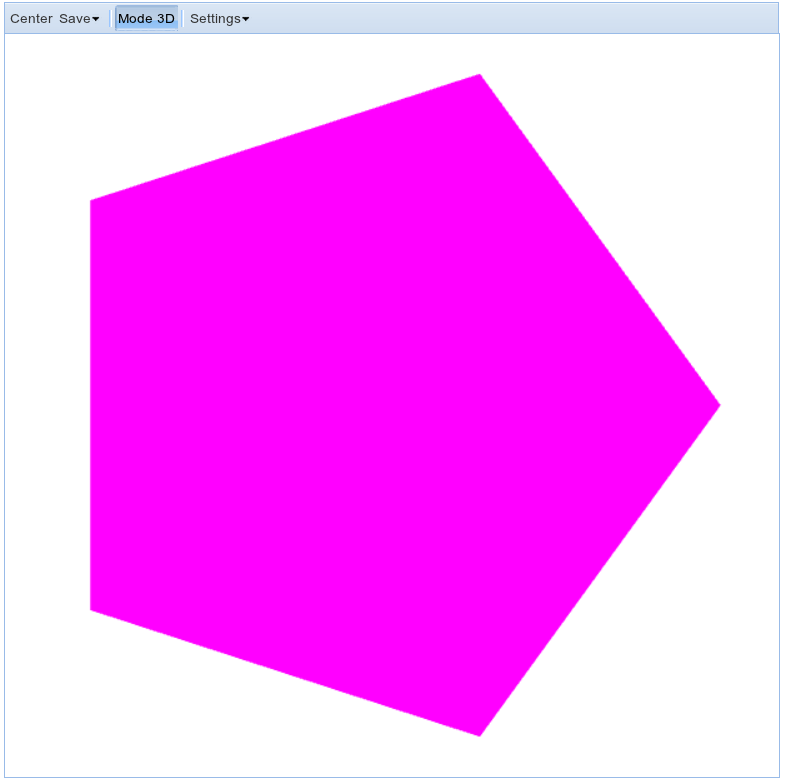
\includegraphics[width=0.5\textwidth]{img/a4-pink-pentagon.png}
\end{center}
\vspace{-4mm}
\caption{Illustration for Exercise 4.}
\label{fig:a4}
%\vspace{-4mm}
\end{figure}
\newpage

\item Create a cyan cone of radius $R$ and height $H$ that stands on its tip
(the tip is at (0, 0, 0) and the axis of the cone coincides with the 
$z$-axis), as shown in Fig. \ref{fig:a5}.

\begin{figure}[!ht]
\begin{center}
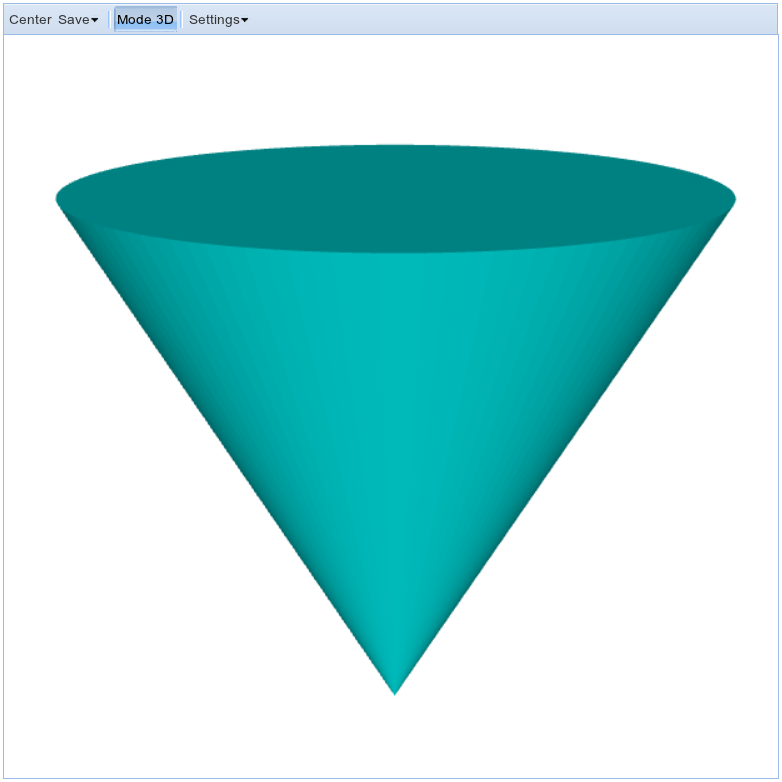
\includegraphics[width=0.5\textwidth]{img/a5-cyan-cone.png}
\end{center}
\vspace{-4mm}
\caption{Illustration for Exercise 5.}
\label{fig:a5}
%\vspace{-1cm}
\end{figure}

\item  Create a carmine cylinder of radius $R$ and height $H$, 
as shown in Fig. \ref{fig:a6}.

\begin{figure}[!ht]
\begin{center}
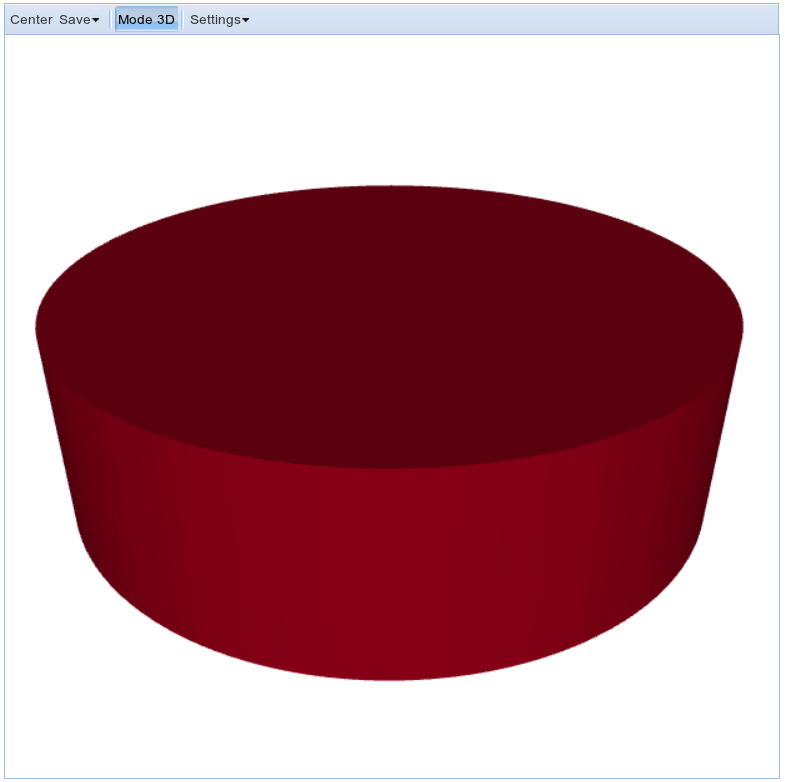
\includegraphics[width=0.5\textwidth]{img/a6-carmine-cylinder.png}
\end{center}
\vspace{-2mm}
\caption{Illustration for Exercise 6.}
\label{fig:a6}
%\vspace{-1cm}
\end{figure}
\newpage

\item Create a topaz tube of inner radius $R_{in}$, outer radius $R_{out}$
and height $H$, as shown in Fig. \ref{fig:a7}.


\begin{figure}[!ht]
\begin{center}
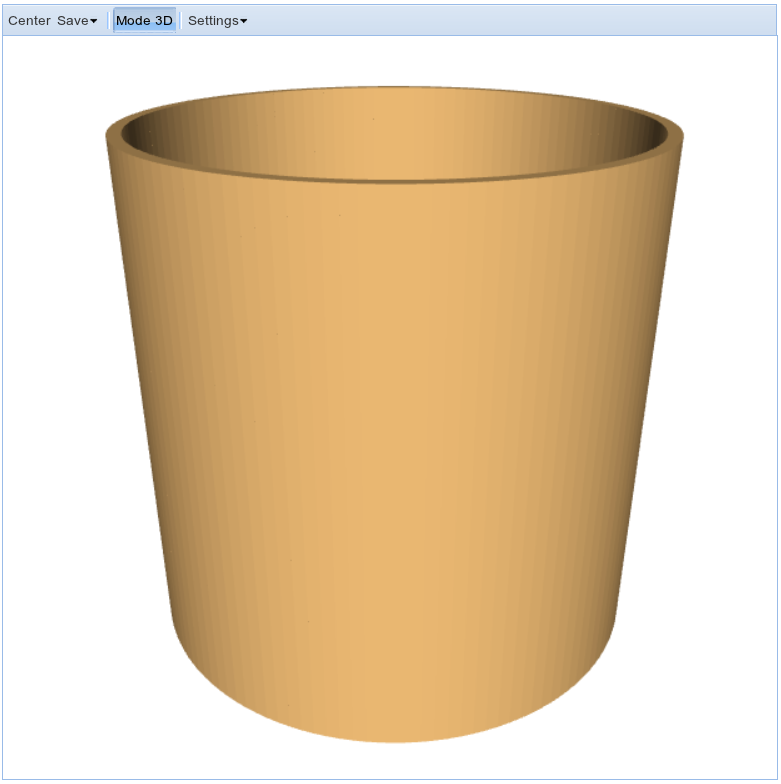
\includegraphics[width=0.5\textwidth]{img/a7-topaz-tube.png}
\end{center}
\vspace{-2mm}
\caption{Illustration for Exercise 7.}
\label{fig:a7}
%\vspace{-1cm}
\end{figure}

\item Create a sand sphere of radius $R$ and center at the origin (0, 0, 0). 
Use $[64, 64]$ for the piecewise-linear approximation of the curved surface, 
as shown in Fig. \ref{fig:a8}.


\begin{figure}[!ht]
\begin{center}
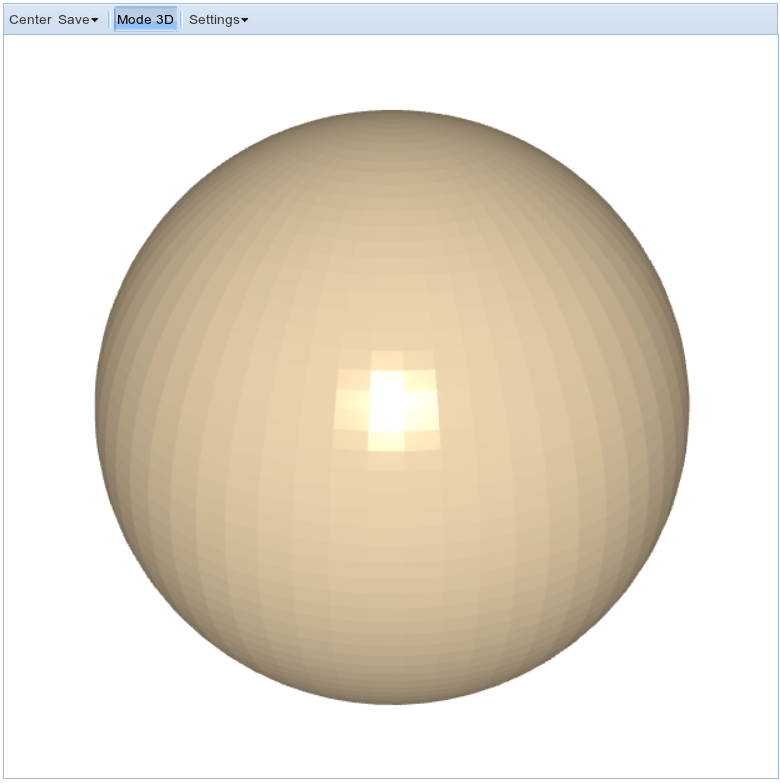
\includegraphics[width=0.5\textwidth]{img/a8-sand-sphere.png}
\end{center}
\vspace{-2mm}
\caption{Illustration for Exercise 8.}
\label{fig:a8}
\vspace{-1cm}
\end{figure}
\newpage

\item Create a turquoise torus of inner radius $R_{in}$ and outer radius $R_{out}$, whose center 
is at the origin (0, 0, 0). Use $[64, 64]$ for the piecewise-linear approximation 
of the curved surface, as shown in Fig. \ref{fig:a9}.


\begin{figure}[!ht]
\begin{center}
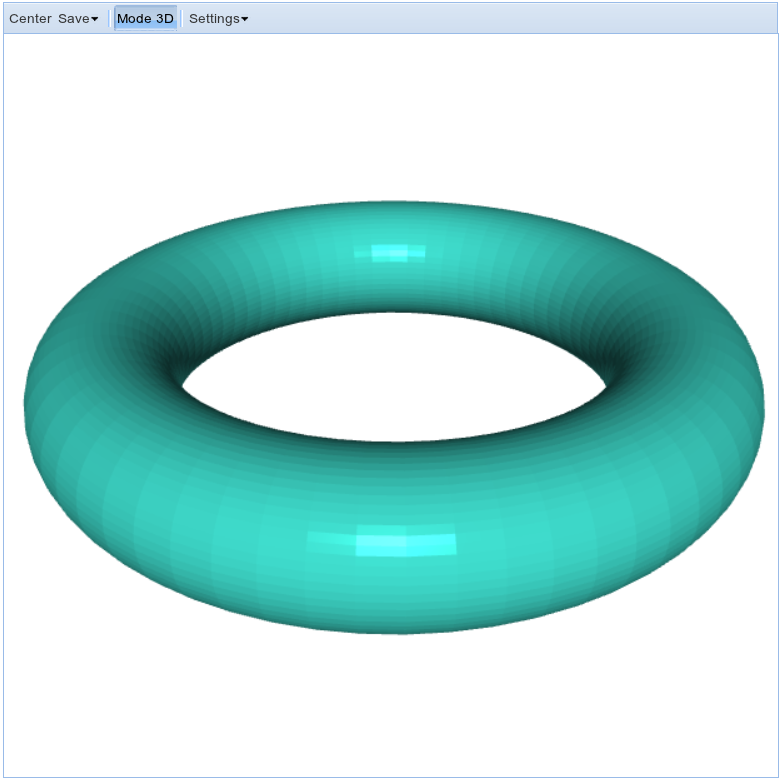
\includegraphics[width=0.5\textwidth]{img/a9-turquoise-torus.png}
\end{center}
\vspace{-2mm}
\caption{Illustration for Exercise 9.}
\label{fig:a9}
%\vspace{-1cm}
\end{figure}

\item Write a script to render a cylinder of radius {\tt R} and height {\tt H}
      via the CONVEXHULL command. The cylinder's axis should coincide with the 
      $z$-axis, the center of its base circle should be (0, 0, 0), and the 
      curved surface should be subdivided into {\tt subdiv} linear segments.

\end{enumerate}

\section{Basic Transformations}

\subsection{Exercises}

\begin{enumerate}
\item 
Create a kitchen table shown in Fig. \ref{fig:b1}. All of its measures should be variable.

\newpage

\begin{figure}[!ht]
\begin{center}
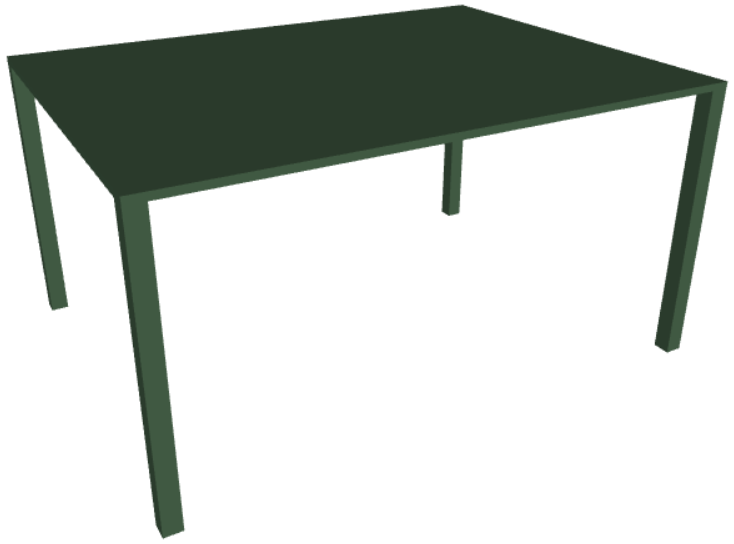
\includegraphics[width=0.5\textwidth]{img/kitchentable.png}
\end{center}
\vspace{-2mm}
\caption{Illustration for Exercise 1.}
\label{fig:b1}
%\vspace{-1cm}
\end{figure}

\item Create a round tea table with round legs as
shown in Fig. \ref{fig:b2}. All of its measures should be variable.

\begin{figure}[!ht]
\begin{center}
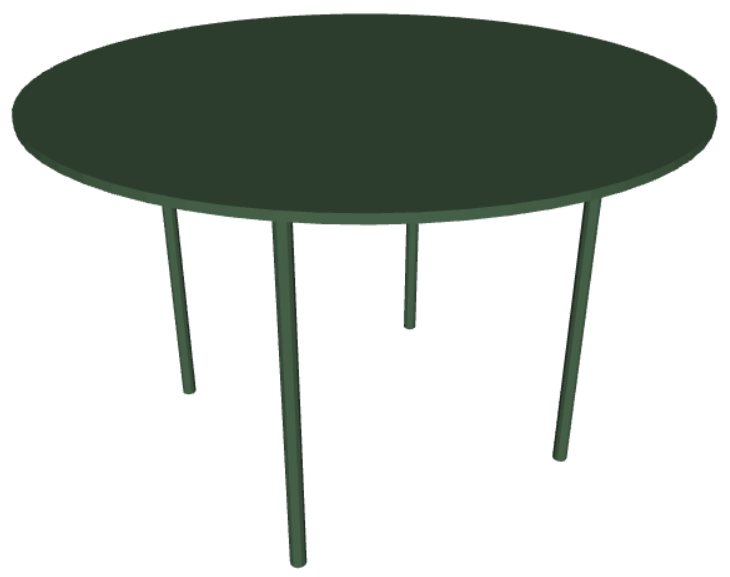
\includegraphics[width=0.5\textwidth]{img/teatable.png}
\end{center}
\vspace{-2mm}
\caption{Illustration for Exercise 2.}
\label{fig:b2}
%\vspace{-1cm}
\end{figure}

\item Use a scaled cylinder and a torus to create a padlock that is shown in Fig. \ref{fig:b3}. 
All of its measures should be variable.

\newpage

\begin{figure}[!ht]
\begin{center}
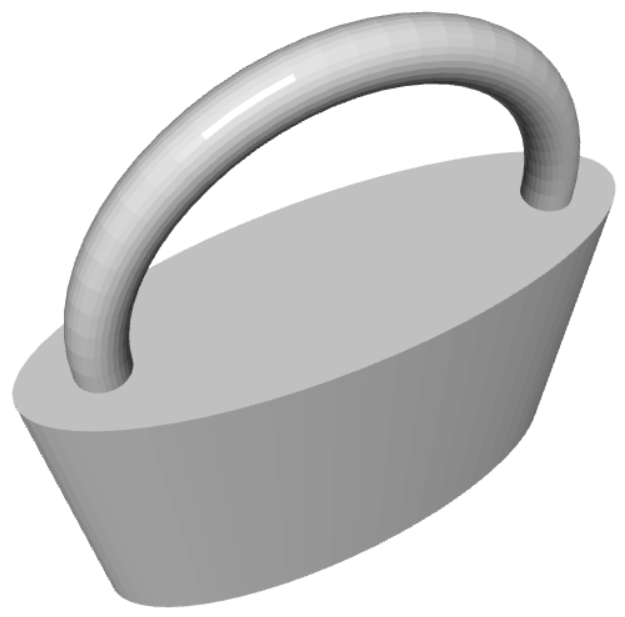
\includegraphics[width=0.4\textwidth]{img/padlock.png}
\end{center}
\vspace{-2mm}
\caption{Illustration for Exercise 3.}
\label{fig:b3}
%\vspace{-1cm}
\end{figure}

\item Use two cylinders and a sphere to create a bottle shown in Fig. \ref{fig:b4}. 
All of its measures should be variable.

\begin{figure}[!ht]
\begin{center}
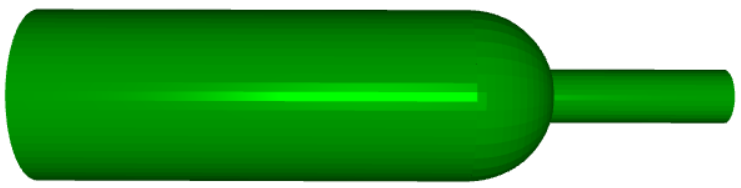
\includegraphics[width=0.8\textwidth]{img/bottle.png}
\end{center}
\vspace{-2mm}
\caption{Illustration for Exercise 4.}
\label{fig:b4}
%\vspace{-1cm}
\end{figure}

\end{enumerate}



\section{Boolean Operations}


\subsection{Exercises}

\begin{enumerate}

\item Use a $4 \times 4 \times 4$ brick to create the object shown in 
Fig. \ref{fig:nclabicon}.

\newpage

\begin{figure}[!ht]
\begin{center}

\includegraphics[width=0.5\textwidth]{img/nclabicon.png}
\end{center}
\vspace{-2mm}
\caption{Illustration for Exercise 1.}
\label{fig:nclabicon}
%\vspace{-1cm}
\end{figure}
\noindent

\item Create a cube and drill three holes into it from the three axial 
directions, as illustrated in Fig. \ref{fig:drilledcube}.
The size of the cube as well as the diameter of the holes should 
be variable. 


\begin{figure}[!ht]
\begin{center}
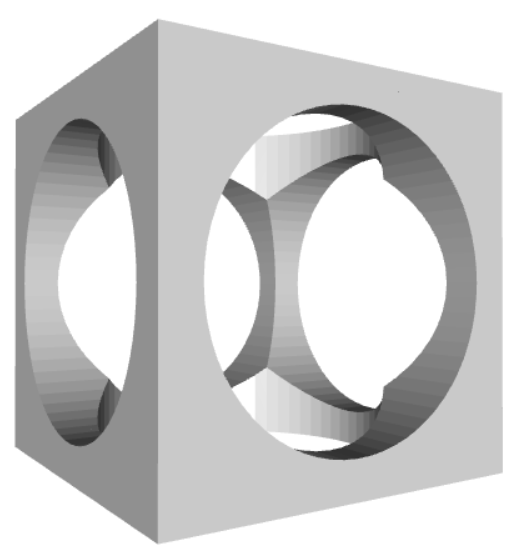
\includegraphics[width=0.4\textwidth]{img/drilledcube.png}
\end{center}
\vspace{-2mm}
\caption{Illustration for Exercise 2.}
\label{fig:drilledcube}
%\vspace{-1cm}
\end{figure}

\item Build a simple model of an ashtray using cylindrical shapes, 
as illustrated in Fig. \ref{fig:ashtray}.
All measures should be variable.

\begin{figure}[!ht]
\begin{center}
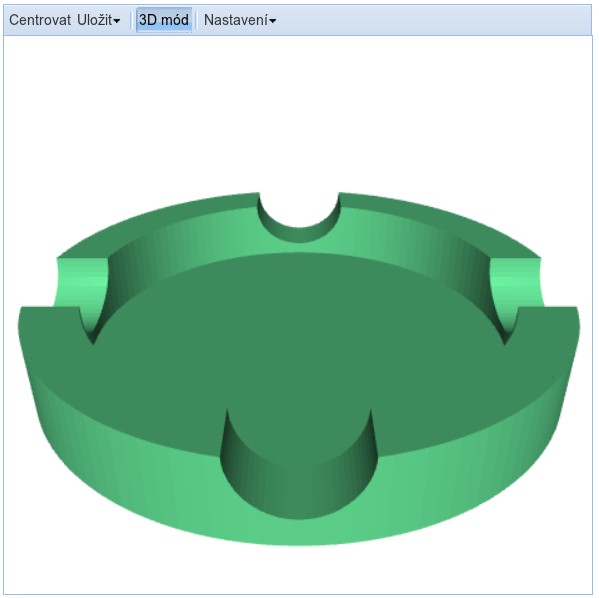
\includegraphics[width=0.5\textwidth]{img/ashtray.png}
\end{center}
\vspace{-2mm}
\caption{Illustration for Exercise 3.}
\label{fig:ashtray}
%\vspace{-1cm}
\end{figure}
\noindent

\end{enumerate}


\section{Creating Simple Objects (Continued)} \label{sec:cso2}


\subsection{Exercises}

Coming soon.


\section{Curves and Curved Surfaces}\label{sec:curves}

\subsection{Exercises}

Coming soon.



\section{The Power of Scripting}

\subsection{Exercises}

\begin{enumerate}
\item Build an Aztec Pyramid as illustrated in Fig. \ref{fig:aztec}. The length 
on the base edge, length of the top edge, height, and the number of layers
should be user-defined parameters. 


\begin{figure}[!ht]
\begin{center}
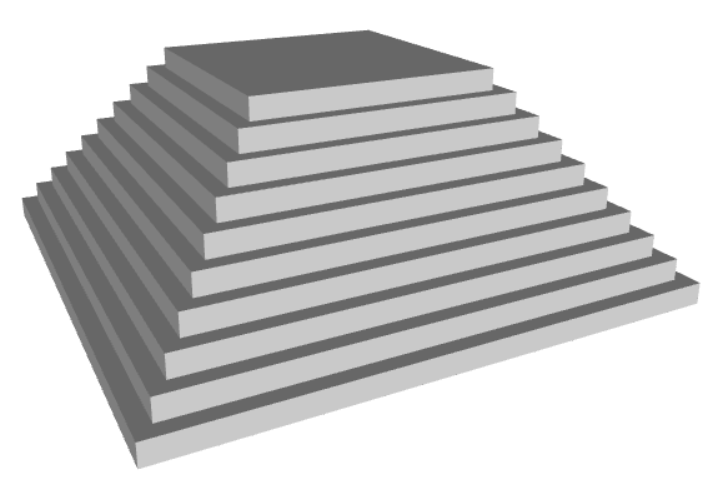
\includegraphics[width=0.7\textwidth]{img/aztec.png}
\end{center}
\vspace{-2mm}
\caption{Illustration for Exercise 1.}
\label{fig:aztec}
%\vspace{-1cm}
\end{figure}
\noindent

\item Build a model of the Tower of Hanoi game as illustrated in Fig. \ref{fig:hanoi}. 
The radius of the largest and smallest disc, and the height of the tower 
should be user-defined parameters. 

\newpage

\begin{figure}[!ht]
\begin{center}
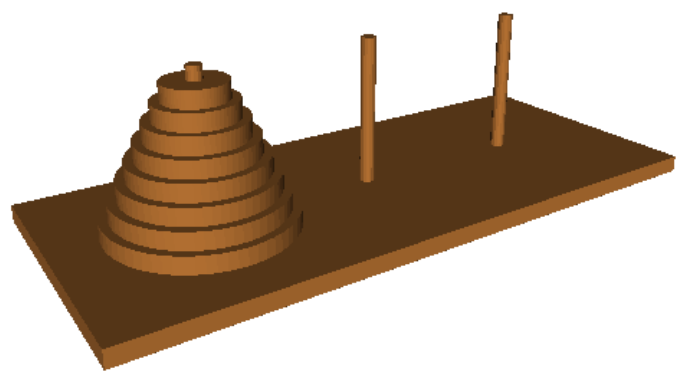
\includegraphics[width=0.7\textwidth]{img/hanoi.png}
\end{center}
\vspace{-2mm}
\caption{Illustration for Exercise 2.}
\label{fig:hanoi}
%\vspace{-1cm}
\end{figure}
\noindent

\item Build a corral for horses with variable radius $r$ and variable number 
of equally-long sides $N$. Also the vertical poles should have general user-defined 
dimensions $W \times W \times H$. Illustrative images of how the corral should look like 
are shown in Fig. \ref{fig:corral2}.

\begin{figure}[!ht]
\begin{center}
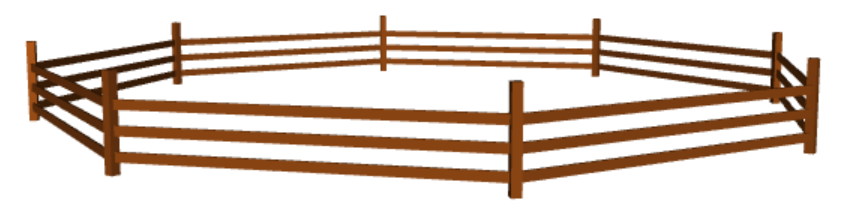
\includegraphics[width=0.7\textwidth]{img/tam-3.png}
\end{center}
\vspace{-2mm}
\caption{Illustration for Exercise 3.}
\label{fig:corral2}
%\vspace{-1cm}
\end{figure}
\noindent

\item Build a spoked wagon wheel similar to the one in Fig. \ref{fig:wheel-1}. All radiuses 
and thicknesses should be user-defined, as well as the number of spokes.

\newpage

\begin{figure}[!ht]
\begin{center}
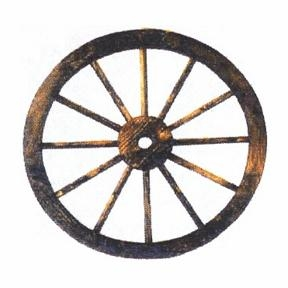
\includegraphics[width=0.5\textwidth]{img/wagonwheel-1.png}
\end{center}
\vspace{-8mm}
\caption{Illustration for Exercise 4.}
\label{fig:wheel-1}
%\vspace{-1cm}
\end{figure}
\noindent

\end{enumerate}



\section{Advanced Techniques}

\subsection{Exercises}

Coming soon.


\end{document}
